%% This is an example first chapter.  You should put chapter/appendix that you
%% write into a separate file, and add a line \include{yourfilename} to
%% main.tex, where `yourfilename.tex' is the name of the chapter/appendix file.
%% You can process specific files by typing their names in at the 
%% \files=
%% prompt when you run the file main.tex through LaTeX.
\chapter{Literature Survey / Framing / Theory}


\section{Development}

\subsection{History and Theory}

Figure \ref{fig:friedman_timeline}; Systems engineering is positioned on the far left of the figure, indicating that the field (or at least the authors listed associated with it) "look to the confirmation and reproduction of existing relationships of power in society. Expressing predominantly technical concerns, they proclaim a carefully nurtured stance of political nuetrality. In reality, they address their work to those who are in power and see their primary mission as serving the state." \cite{mazza2017}

"The engineer's sense of certainty (and his ignorance of history) informed some of the most prominent of later planning theorists... all of whome were enthralled by the idea of "designing society" \cite{mazza2017}

"There was a moment in time when aeronautic and space engineers throught that, having reached the moon, they could now turn their energies to solving hte problem of growing violence in cities along with other urban "crises." \cite{mazza2017}

\clearpage
\begin{sidewaysfigure}[t]
	\centering
	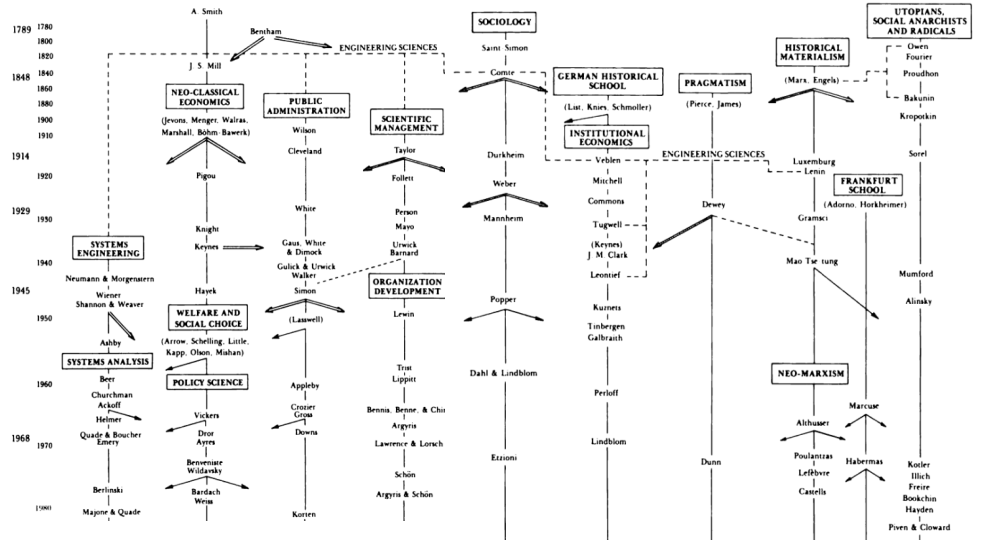
\includegraphics[scale=0.65]{Figures/chap2/friedman_timeline.png}
	\caption{Timeline of intellectual influences on American planning theory. From \cite{mazza2017}}
	\label{fig:friedman_timeline}
\end{sidewaysfigure}
\clearpage

Also use diagram/framework from \cite{marcuseThreeHistoricCurrents2016}:

\begin{itemize}
    \setlength{\itemsep}{0pt}%
    \setlength{\parskip}{0pt}%
	\item{\textbf{Technicist:} Planning focused on maximizing efficient of the system being planned. The planner is a technical professional with specialized knowledge. The "technicist is inherently conservative: it is to serve an economic and social and policital order in which its role is to make that order function smoothly."}
	\item{\textbf{Social Reform:} Planning grounded in social ideas and values while viewing the necessary changes as possible within the exisiting framework of social, political, and economic order. The exact values of concern have varied over the years, with environmental sustainability coming to the rise more recently.}
	\item{\textbf{Social Justice:} Planning by grass-roots groups and social movements, putting values ahead of efficiency, and willing to work outside of existing systems to accomplish its goals.}
\end{itemize}


\begin{table}[h]
\caption{Axes of currents of city planning. Based on  \cite{marcuseThreeHistoricCurrents2016}}
\label{table:currents}
\begin{center}
\begin{tabular}{| C{0.1cm} C{0.1cm} | C{2cm} | C{3cm} | C{3cm} |} \cline{4-5}

\multicolumn{1}{c}{} & \multicolumn{1}{c}{} & \multicolumn{1}{c|}{} & \multicolumn{2}{c|}{\textit{Stance towards existing relations of power}}  \\ \cline{4-5}

\multicolumn{1}{c}{} & \multicolumn{1}{c}{} & \multicolumn{1}{c|}{} & \textbf{Critical} & \textbf{Deferential} \\ \hline

\multirow{4}{*}{\parbox{4cm}{\rotatebox[origin=c]{90}{\textit{Primary}}}}
& \multirow{4}{*}{\parbox{4cm}{\rotatebox[origin=c]{90}{\textit{concern}}}} 
& \multirow{2}{*}{\textbf{Social}} 
& \multirow{2}{*}{Social Justice} 
& \multirow{2}{*}{Social Reform} \\ 

& & & & \\ \cline{3-5}

& & \multirow{2}{*}{\textbf{Efficiency}} & & \multirow{2}{*}{Technicist} \\

& & & & \\  \hline

\end{tabular}
\end{center}
\end{table}



"The systems engineers bring some expertise and substantial pretensions to the problems of the city. Their prinicpal system expertise seems to be relative to complex organizations that are mission oriented. There is in any case a good deal of difference between the mission of reaching the moon, and the mission of surival and welfare for soceity and the city. The systems engineer can in general deal best with subsystems and specific tasks, and he therefore suboptimizes. This is a charitable description." \cite{robinsonDecisionmakingUrbanPlanning1972}



Respond to critiques of central planning / technocratic efforts by Easterly \cite{easterly2015}

Planning has come a long way from focusing on single page map and a timescale of 20-30 years (Section 2 Introduction of \cite{robinsonDecisionmakingUrbanPlanning1972})

By providing tools for more participation, we are not necessarily doing anything radical. "Democracies rarely end up expropriating and redistributing capital" \cite{fainsteinSpatialJusticePlanning2016}. "Participation is not power; its reform is not radical" \cite{marcuseThreeHistoricCurrents2016}. Some argue that neoliberalism in factor prefers to use participation as a means of underming resistance, rather than violence, though this has the risk of providing a structure for coalition building and radicalization \cite{miraftabInsurgentPlanningSituating2016}. In fact, increased community involvement can result in more restrictive, unambitious goals that are not in the interests of certain minorities (Section 1, Chapter 2 of \cite{robinsonDecisionmakingUrbanPlanning1972}).

\subsection{Sustainable Development}

"The pessimistic thought is that sustainable development has been stripped of its transformative power and reduced to its lowest common demoninator. After all, if both the World Bank and radical ecologists now believe in sustainability, the concept can have no teeth: it is so malleable as to mean many things to manny people without requiring commitment to any specific policies." \cite{campbellGreenCitiesGrowing2016}

"Yet there is also an optimistic interpretation of the broad empbrace given sustainability: the idea has become hegemonic, an accepted meta-narrative, a given. It has shifted from being a variable to being the parameter of hte debate, almost certain to be integrated into any future scenario of development." \cite{campbellGreenCitiesGrowing2016}

"To... critics, the prospect of integrating economic, environmental and equity interests will seem forced and artificial. States will require communities to prepare "Sustinable Development Master Plans," which will prove to be glib wish lists of goals and suspiciously vague implementation steps. To achieve consensus for the plan, language wil lbe reduced to the lowest common demoninator, and the pleasing plans will gather dust." (written in 1996, pre MDGs and SDGs) \cite{campbellGreenCitiesGrowing2016}

"The danger of translation is that one language will dominate the debate and thus define the terms of the solution. It is essential to exert equal effort to translate in each direction, to prevent one linguistic culture from dominating the other... Another lesson from the neocolonial inguistic experience is that it is crucial for each social group to express itself in its own language before any translation. The challenge for planners is to write the best translations among the languages of the economic, the ecological, and the social views, and to avoid a quasi-colonial dominance by the economic \textit{ingua franca}, by creating equal two-way translations... Translation can thus be a powerful planner's skill, and interdisciplinary planning education already provides some multiculturalism. Moreover, the idea of sustainability lends itself nicely to the meeting on common ground of competing value systems." \cite{campbellGreenCitiesGrowing2016}




\begin{figure}[h]
	\centering
	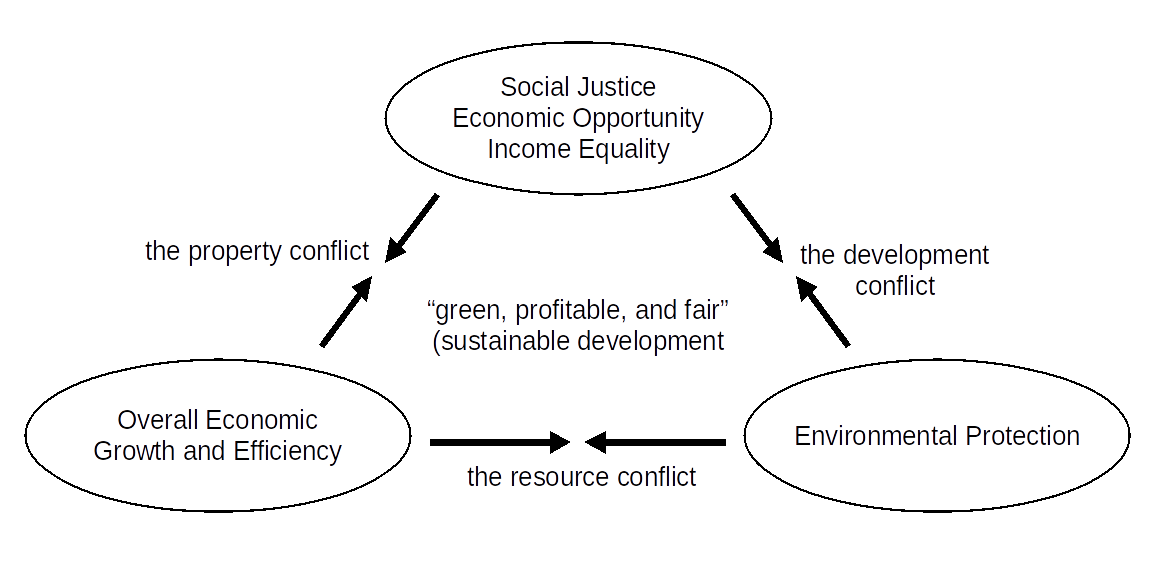
\includegraphics[scale=0.35]{Figures/chap2/sustainable_triangle.png}
	\caption{The triangle of conflicting goals of sustainable development. Adapted from \cite{campbellGreenCitiesGrowing2016}}
	\label{fig:sustainable_triangle}
\end{figure}


Talk about \acp{mdg} and \acp{sdg}, pull from my previously written articles, also \cite{unitednationsWhoWillBe2013}

Respond to critiques of \acp{mdg}/\acp{sdg} \cite{alstonShipsPassingNight2005, reddyGlobalDevelopmentGoals2008}

\subsection{GIS in development}

\ac{pgis}: Refer to macro-micro framework from Table 2.1, pg.17. What parts this thesis covers and what parts we envision EVDT covering in the long term. Also refer to EAST2 model on pg. 21 \cite{jankowskiGISGroupDecision2001}

\begin{table}[h]
\caption{Generic macro-micro, participtory decision strategy. Adapted from \cite{jankowskiGISGroupDecision2001}}
\label{table:macro-micro}
\begin{center}
\begin{tabular}{ L{3cm} L{4cm}  L{4cm} L{4cm}} \hline
& \multicolumn{3}{c}{\textit{Macro-phases in a decision strategy}}  \\ \cline{2-4}

\textit{Micro-activities in a decision strategy} & \textbf{\textit{1. Intelligence}} about values, objectives, and criteria & \textbf{\textit{2. Design}} of a set of feasible options &  \textbf{\textit{3. Choice}} about recommendations \\ \hline

\textbf{A. Gather...} & issues to develop and refine \textbf{value trees} as a basis for objectives & \textbf{primary criteria} as a basis for option generation & \textbf{values, criteria, and option list scenarios} for an evaluation \\ \hline

\textbf{B. Organize...} & \textbf{ojbectives} as a basis for criteria and constraints & and apply approaches(es) for \textbf{option generation} & approaches to \textbf{priority and sensitivity analyses} \\ \hline

\textbf{C. Select...} & \textbf{criteria} to be used in analysis as a basis for generating options & the \textbf{feasible option list} & \textbf{recommendation} as a prioritized list of options \\ \hline

\textbf{D. Review...} & criteria, \textbf{resources, constraints,} and \textbf{standards} & \textbf{option set(s)} in line with resources, constraints, and standards & \textbf{recommendation(s)} in line with original \textbf{value(s), goal(s),} and \textbf{objectives} \\ \hline

\end{tabular}
\end{center}
\end{table}

\begin{figure}[h]
	\centering
	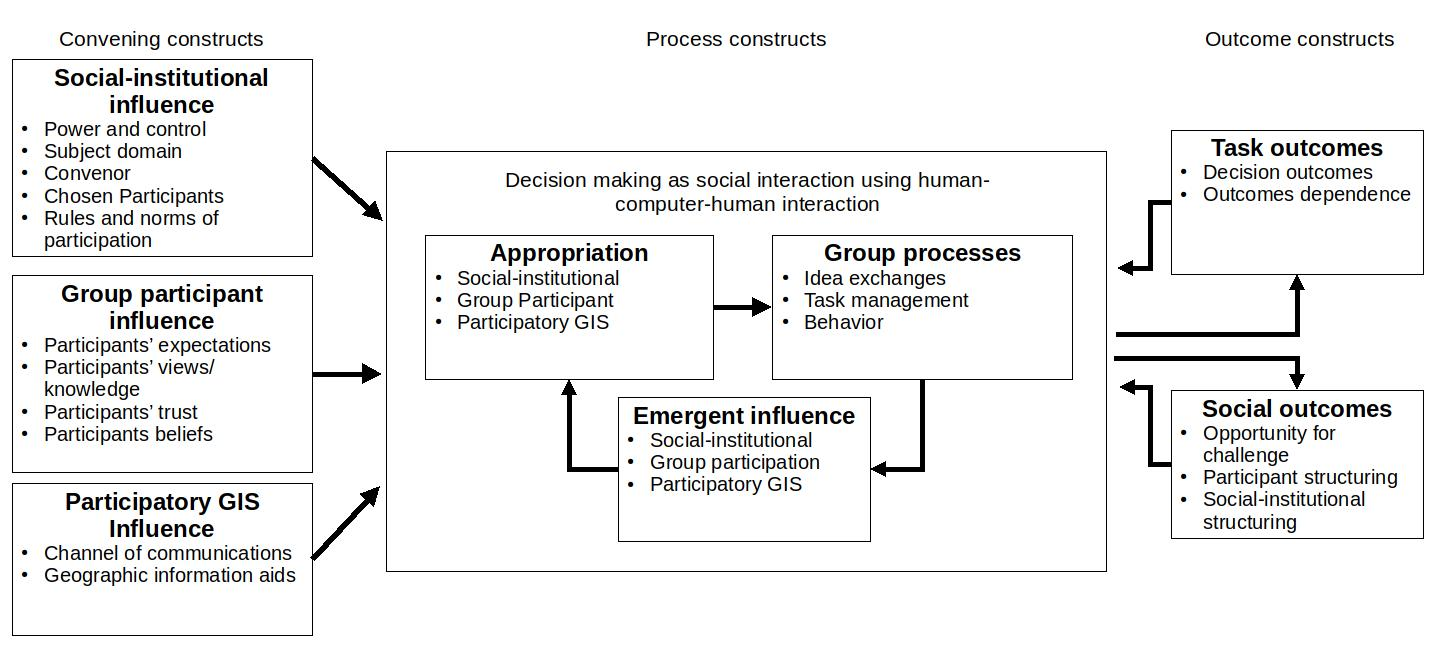
\includegraphics[scale=0.4]{Figures/chap2/east2.jpg}
	\caption{Enhanced Adaptive Structuration Theory 2 (EAST2). Adapted from \cite{jankowskiGISGroupDecision2001}}
	\label{fig:east2}
\end{figure}


Jankowski and Nyerges lay out seven common design requirements for spatial decision support tools \cite{jankowskiGISGroupDecision2001}:

\begin{enumerate}
    \setlength{\itemsep}{0pt}%
    \setlength{\parskip}{0pt}%
	\item{A spatial decision support system for collaborative work should offer decisional guidance to users in the form of an agenda.}
	\item{A system should not be restrictive, allowing the users to select tools and procedures in any order.}
	\item{A system should be comprehensive within the realm of spatial decision problems, and thus offer a number of decision space exploration tools and evaluation techniques.}
	\item{The user interface should be both process-oriented and data-oriented to allow an equally easy access to task-solving techniques, as well as maps and data visualization tools.}
	\item{A system should be capable of supporting facilitated meetings and hence, allow for the information exchange to proceed among group members, and between group members and the facilitator. It should also allow space- and time-distributed collaborative work by facilitating information exchange, electronic submission of solution options, and voting through the internet.}
	\item{A system functionality should include extensive multiple criteria evaluation capabilities, sensitivity analysis, specialized maps to support the enumeration of preferences and comparison of alternative performance, voting, and consensus building tools.}
	\item{A system should provide ncessary functionality to support needs of an advanced user without overwhelming a novice who needs a user-guiding interface.}
\end{enumerate}


the meeting arrangment that EVDT supports, \ref{table:meeting_arrangements}

\begin{table}[h]
\caption{Different types of meeting arrangements. Adapted from \cite{jankowskiGISGroupDecision2001}}
\label{table:meeting_arrangements}
\begin{center}
\begin{tabular}{ L{3cm} L{5.5cm}  L{5.5cm}}  \hline
 & \textit{Same time} &\textit{Different time}  \\ \cline{2-3}
\textbf{\textit{Same place}} & \textbf{Conventional Meeting} \qquad \textit{Advantage:} 
\vspace{-5mm}
\begin{itemize}
    \setlength{\itemsep}{0pt}%
    \setlength{\parskip}{0pt}%
	\item{face-to-face expressions}
	\item{immediate response}
\end{itemize} &
\textbf{Storyboard meeting} \qquad \textit{Advantage:} 
\vspace{-5mm}
\begin{itemize}
    \setlength{\itemsep}{0pt}%
    \setlength{\parskip}{0pt}%
	\item{scheduling is easy}
	\item{respond anytime}
	\item{leave-behind note}
\end{itemize} 
\\
& \textit{Disadvantage:} 
\vspace{-5mm}
\begin{itemize}
    \setlength{\itemsep}{0pt}%
    \setlength{\parskip}{0pt}%
	\item{scheduling is difficult}
\end{itemize} &
\textit{Disadvantage:} 
\vspace{-5mm}
\begin{itemize}
    \setlength{\itemsep}{0pt}%
    \setlength{\parskip}{0pt}%
	\item{meeting takes longer}
	\item{difficult to maintain in the long run}
\end{itemize} 
\\ \hline

\textbf{\textit{Different place}} & \textbf{Conference call meeting} \qquad \textit{Advantage:} 
\vspace{-5mm}
\begin{itemize}
    \setlength{\itemsep}{0pt}%
    \setlength{\parskip}{0pt}%
	\item{no need to travel}
	\item{immediate response}
\end{itemize} &
\textbf{Distributed meeting} \qquad \textit{Advantage:} 
\vspace{-5mm}
\begin{itemize}
    \setlength{\itemsep}{0pt}%
    \setlength{\parskip}{0pt}%
	\item{scheduling is convenient}
	\item{no need to travel}
	\item{submit response anytime}
\end{itemize} 
\\
& \textit{Disadvantage:} 
\vspace{-5mm}
\begin{itemize}
    \setlength{\itemsep}{0pt}%
    \setlength{\parskip}{0pt}%
	\item{limited personal perspective from participants}
	\item{meeting protocols are difficult to interpret}
	\item{difficult to maintain meeting dynamics}
\end{itemize} &
\textit{Disadvantage:} 
\vspace{-5mm}
\begin{itemize}
    \setlength{\itemsep}{0pt}%
    \setlength{\parskip}{0pt}%
	\item{meeting takes longer}
	\item{meeting dynamics are different from normal meeting ("netiquette" instead of face-to-face etiquette)}
\end{itemize} 
\\ \hline
\end{tabular}
\end{center}
\end{table}

Levels of decision support \cite{jankowskiGISGroupDecision2001}:

\begin{enumerate}[itemsep=0pt,parsep=0pt]
	\item{\textit{Basic information handling support}}
%	\vspace{-5mm}
		\begin{enumerate}[itemsep=0pt,parsep=0pt,topsep=0pt, partopsep=0pt]
			\item{Information management}
			\item{Visual aids}
			\item{Group collaboration support}
		\end{enumerate}
%	\vspace{-5mm}
	\item{\textit{Decision Analysis Support}}
%	\vspace{-5mm}
		\begin{enumerate}[itemsep=0pt,parsep=0pt,topsep=0pt, partopsep=0pt]
			\item{Option modeling}
			\item{Choice models}
			\item{Structured group process techniques}
		\end{enumerate}
%	\vspace{-5mm}
	\item{\textit{Group reasoning support}}
%	\vspace{-5mm}
		\begin{enumerate}[itemsep=0pt,parsep=0pt,topsep=0pt, partopsep=0pt]
			\item{Judgement refinement/amplification techniques}
			\item{Analytical reasoning methods}
		\end{enumerate}
\end{enumerate}

\subsection{[Tentative] Informality}
Discuss and critique of informality as a concept \cite{royUrbanInformalityProduction2016}

De Soto argues that the poor already have assets, just needs to be formalized. \cite{sotoMysteryCapitalWhy2003} though others argue that this is just results in a cycle of appeasment / welfare \cite{hollandForbearanceRedistributionPolitics2017}


\section{Types of places that EVDT deals with}

Commonly has to do with \acp{cpr}. Talk about the three common ways of managing \acp{cpr}: Central management, privatization, self-management. Bring in Table \ref{table:cpr_design}  showing design principles of long-enduring self-management institutions. Refer to successful aspects of the water basin in California (incremental and sequential process to reduce the costs of local institutional supply, shared information at each step, intermediate benefits from initial investments were realized prior to larger investments, transformed structure of incentives within which fuure strategic decisions can be made) (pg. 137. \cite{ostromGoverningCommonsEvolution2015}

\begin{table}[h]
\caption{Design principles illustrated by long-lasting \ac{cpr} institutions. Adapted from \cite{ostromGoverningCommonsEvolution2015}}
\label{table:cpr_design}
\begin{center}
\begin{tabular}{ L{0.5cm} L{8cm}} \hline
1. & Clearly defined boundaries \\
2. & Congruence between appropriation and provision rules and local conditions \\
3. & Collective-choice arrangements \\
4. & Monitoring \\
5. & Graduated sanctions \\
6. & Conflict-resolution mechanisms \\
7. & Minimal recognition of rights to organize \\
\multicolumn{2}{l}{\textit{For CPRs that are parts of larger systems:}} \\
8. & Nested enterprises \\ \hline
\end{tabular}
\end{center}
\end{table}

\section{Complex Systems and Modeling}

The growth and development of cities is a complex system. Much work has been done using cellular automata and fractals to model them \cite{battyCitiesComplexity2005}

Urban planners have been seeking to develop useful indices and indicators akin to those used in engineering and remote observation contexts for decades (Section 1, Cahpter 3 of \cite{boyceFrameworkDefiningApplying1972}


"Futures planning as described and prescribed by futurists is different from planning \textit{for} te future; it is an attempt to manipulate or plan \textit{the} future. A basic characteristic of this orientation is the use of such terms as "designing," "inventing," or even "making" the future. When the future is being planned for, rather than designed, the implication is that the planner is trying to make specific and limited accomodations to the broad and overall characteristics of the future he considers either immutable or too formidable to be fundamentally rearranged or restructured." \cite{robinsoniraPlanFormulationIntroductoryNote1972}

"If alternatives are not carefully related to goals and objectives there is the real danger that they will either fail to reflect certain important issues which the planning process to being used to study, or worse still, be almost irrelevant... Alternatives must reflect the goals sought; the means must reflect the ends." \cite{mcloughlinChartingPossibleCourses1972}



Position \ac{evdt} using the different dimensions of models proposed in \cite{harrisQuantitativeModelsUrban1972}:

\begin{enumerate}[itemsep=0pt,parsep=0pt]
	\item{descriptive vs. analytic}
	\item{holistic vs. partial}
	\item{macro vs. micro}
	\item{static vs. dynamic}
	\item{deterministic vs. probabilistic}
	\item{simultaneous vs. sequential (directly calculate the output or go through intermediate phases)}
\end{enumerate}


In order for cost-benefit analysis to maximize economic welfare, the following conditions must be met \cite{krutillaWelfareAspectsBenefitCost1961}:

\begin{enumerate}[itemsep=0pt,parsep=0pt]
	\item{Opportunity costs are borne by beneficiaries in  such wise as to retain the initial income distribution}
	\item{The initial income distribution is in some sense "best}
	\item{The marginal social rates of transformation between any two commodities are everywhere equal to their corresponding rates of substitution except for the area(s) justifying the intervention in question}
\end{enumerate}

More details modeling, as well as breaking down specific costs and benefits (as opposed to converting them to monetary terms and summing them) and attributing them to specific goals, can circumvent these constraints, though at the cost of increased complexity \cite{hillGoalsAchievementMatrixEvaluating1972}.

This work does not directly incorporate mechanisms for multi-stakeholder negotiation or tradespace exploration, but it is amenable to extension with such mechanisms (refer to SEAri research)

The Law of requisite variety from the field of cybernetics says that the variety (the number of elements or states) of the control device must be at least equal to that of the disturbances \cite{ashbyRequisiteVarietyIts1991}. Any development plan is going to fall far short of the variety expressed by human society and the natural environment. Planning efforts must then make reliance on the natural homeostasis behavior of such systems and of more flexible, ad hoc measures not specified in the plan in order to make up the difference in variety. \cite{mcloughlinSystemGuidanceControl1972}


\section{EVDT Framework}

Is not itself a means of planning and implementing projects. It is not a full life-cycle tool such as \ac{ppbs} \cite{hatryCriteriaEvaluationPlanning1972}

%\section{Section sample 1}


%\begin{enumerate}
%  \item Item 1.
%  \item Item 2.
%  \item Item 3.
%\end{enumerate}
%
%
%
%\begin{eqnarray*}
%a_i & = & a_j + a_k \\
%a_i & = & 2a_j + a_k \\
%a_i & = & 4a_j + a_k \\
%a_i & = & 8a_j + a_k \\
%a_i & = & a_j - a_k \\
%a_i & = & a_j \ll m \mbox{shift}
%\end{eqnarray*}
%instead of the multiplication.  For example, you could use:
%\begin{eqnarray*}
%r & = & 4s + s\\
%r & = & r + r
%\end{eqnarray*}
%Or by xx:
%\begin{eqnarray*}
%t & = & 2s + s \\
%r & = & 2t + s \\
%r & = & 8r + t
%\end{eqnarray*}
